\documentclass[seminar,palatino]{AIGpaper}
% Please read the README.md file for additional information on the parameters and overall usage of AIGpaper

%%%% Package Imports %%%%%%%%%%%%%%%%%%%%%%%%%%%%%%%%%%%%%%%%%%%%%%%%%%%%%%%%%%%%%%%%%
\usepackage{graphicx}					    % enhanced support for graphics
\usepackage{tabularx}				      	% more flexible tabular
\usepackage{amsfonts}					    % math fonts
\usepackage{amssymb}					    % math symbols
\usepackage{amsmath}					    % overall enhancements to math environment

%%%% optional packages
\usepackage{tikz}                           % creating graphs and other structures
\usetikzlibrary{arrows,positioning}
\tikzset{
    %Define standard arrow tip
    >=stealth',
    %Define style for argument
    args/.style={circle, minimum size=0.9cm,draw=black, thick,fill=white},
}


%%%% Author and Title Information %%%%%%%%%%%%%%%%%%%%%%%%%%%%%%%%%%%%%%%%%%%%%%%%%%%
\author{Erika Mustermann}

\title{Die Verbreitung des Begriffes \glqq{}Mustermann\grqq{} im Zusammenhang mit Beispieltexten}


%%%% Abstract %%%%%%%%%%%%%%%%%%%%%%%%%%%%%%%%%%%%%%%%%%%%%%%%%%%%%%%%%%%%%%%%%%%%%%

\germanabstract{
Lorem ipsum dolor sit amet, consetetur sadipscing elitr, sed diam nonumy eirmod tempor invidunt ut labore et dolore magna aliquyam erat, sed diam voluptua. At vero eos et accusam et justo duo dolores et ea rebum. Stet clita kasd gubergren, no sea takimata sanctus est Lorem ipsum dolor sit amet. Lorem ipsum dolor sit amet, consetetur sadipscing elitr, sed diam nonumy eirmod tempor invidunt ut labore et dolore magna aliquyam erat, sed diam voluptua.
}

% use this if the document is written in english
%\englishabstract{}


\begin{document}

\maketitle % prints title and author information, as well as the abstract 


% ===================== Beginning of the actual text section =====================

\section{Lorem Ipsum}
Lorem ipsum dolor sit amet, consetetur sadipscing elitr, sed diam nonumy eirmod tempor invidunt ut labore et dolore magna aliquyam erat, sed diam voluptua. At vero eos et accusam et justo duo dolores et ea rebum. Stet clita kasd gubergren, no sea takimata sanctus est Lorem ipsum dolor sit amet. Lorem ipsum dolor sit amet, consetetur sadipscing elitr, sed diam nonumy eirmod tempor invidunt ut labore et dolore magna aliquyam erat, sed diam voluptua. At vero eos et accusam et justo duo dolores et ea rebum. Stet clita kasd gubergren, no sea takimata sanctus est Lorem ipsum dolor sit amet. Lorem ipsum dolor sit amet, consetetur sadipscing elitr, sed diam nonumy eirmod tempor invidunt ut labore et dolore magna aliquyam erat, sed diam voluptua. At vero eos et accusam et justo duo dolores et ea rebum. Stet clita kasd gubergren, no sea takimata sanctus est Lorem ipsum dolor sit amet.   

Duis autem vel eum iriure dolor in hendrerit in vulputate velit esse molestie consequat, vel illum dolore eu feugiat nulla facilisis at vero eros et accumsan et iusto odio dignissim qui blandit praesent luptatum zzril delenit augue duis dolore te feugait nulla facilisi. Lorem ipsum dolor sit amet, consectetuer adipiscing elit, sed diam nonummy nibh euismod tincidunt ut laoreet dolore magna aliquam erat volutpat.   


\section{Example Figures and Tables}
Figure \ref{fig:af} shows an example of an abstract argumentation framework \cite{dung1995acceptability}.

\begin{figure}[ht]
    \centering
    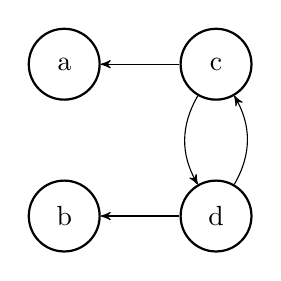
\begin{tikzpicture}[node distance=1cm]
    	\node[args](args1){a};
    	\node[args, below=of args1](args2){b};
    	\node[args, right=of args1](args3){c};
    	\node[args, right=of args2](args4){d};
    
        \path(args3) edge [->] (args1);
        \path(args3) edge [->, bend right] (args4);
        \path(args4) edge [->, bend right] (args3);
    	\path(args4) edge [->] (args2);
    \end{tikzpicture}
    \caption{An abstract argumentation framework.}
    \label{fig:af}
\end{figure}


\begin{table*}[ht]
\begin{center}
\begin{tabular}{lll}
\hline
1&2&3\\
4&5&6\\
\hline
\end{tabular}
\end{center}
\caption{Table caption.} \label{tab:t1}
\end{table*}



\subsection{Encoding Test}
Städte, Länder, Flüsse


% References
\addreferences

\makestatement{1}

\end{document}
